%-------%%%%%%%% PREPARE FOR THE ABSTRACT BIBLIOGRAPH FIG. AND TAB. %%%%%%%%-----------%
%
%\begin{CJK}{UTF8}{gbsn} %针对文字编码为unix %CJK自带的utf-8简体字体有gbsn(宋体)和gkai(楷体)
%\begin{CJK}{GBK}{hei}	%针对文字编码为doc
%\begin{CJK}{GBK}{hei}	 %针对文字编码为doc
%\CJKindent     %在CJK环境中,中文段落起始缩进2个中文字符
%\indent
%
\renewcommand{\abstractname}{\small{\CJKfamily{hei} 摘\quad 要}} %\CJKfamily{hei} 设置中文字体,字号用\big \small来设
\renewcommand{\contentsname}{\centering\CJKfamily{hei} 目~~~录}
\renewcommand{\refname}{\centering\CJKfamily{hei} 主~要~参~考~资~料}
%\renewcommand{\figurename}{\CJKfamily{hei} 图.}
%\renewcommand{\figurename}{{\bf Fig}.}
\renewcommand{\figurename}{}
%\renewcommand{\tablename}{\CJKfamily{hei} 表.}
\renewcommand{\tablename}{{\bf Tab}.}
%\renewcommand{\thesubfigure}{\roman{subfigure}}  \makeatletter %子图标记罗马字母
%\renewcommand{\thesubfigure}{\tiny(\alph{subfigure})}  \makeatletter %子图标记英文字母
%\renewcommand{\thesubfigure}{}  \makeatletter %子图无标记
%
\newcommand{\keywords}[1]{{\hspace{0pt}\small{\CJKfamily{hei} 关键词:}{\hspace{2ex}{#1}}\bigskip}}
%%将图表的Caption写成 图(表) Num. 格式
%\makeatletter
%\long\def\@makecaption#1#2{%
%  \vskip\abovecaptionskip
%  \sbox\@tempboxa{#1. #2}%
%  \ifdim \wd\@tempboxa >\hsize
%    #1. #2\par
%  \else
%    \global \@minipagefalse
%    \hb@xt@\hsize{\hfil\box\@tempboxa\hfil}%
%  \fi
%  \vskip\belowcaptionskip}
%\makeatother
%
%----------------------------------------------------------------------------------------------------------------------------------------------------%
%
%------%%%%%%%%%%%%%%------The Abstract and the keywords of The Paper-------%%%%%%%%%%%%%--------%

%\begin{abstract}
%The content of the abstract
%\end{abstract}

%\keywords{Keyword1; Keyword2; Keyword3}

%----------------------------------------------------------------------------------------------------------------------------------------------------%

\newpage
\pagestyle{empty}    % 清空页码                                      %
\vskip -0.3in
\begin{figure}[h!]
\centering
\hspace*{4.5in}
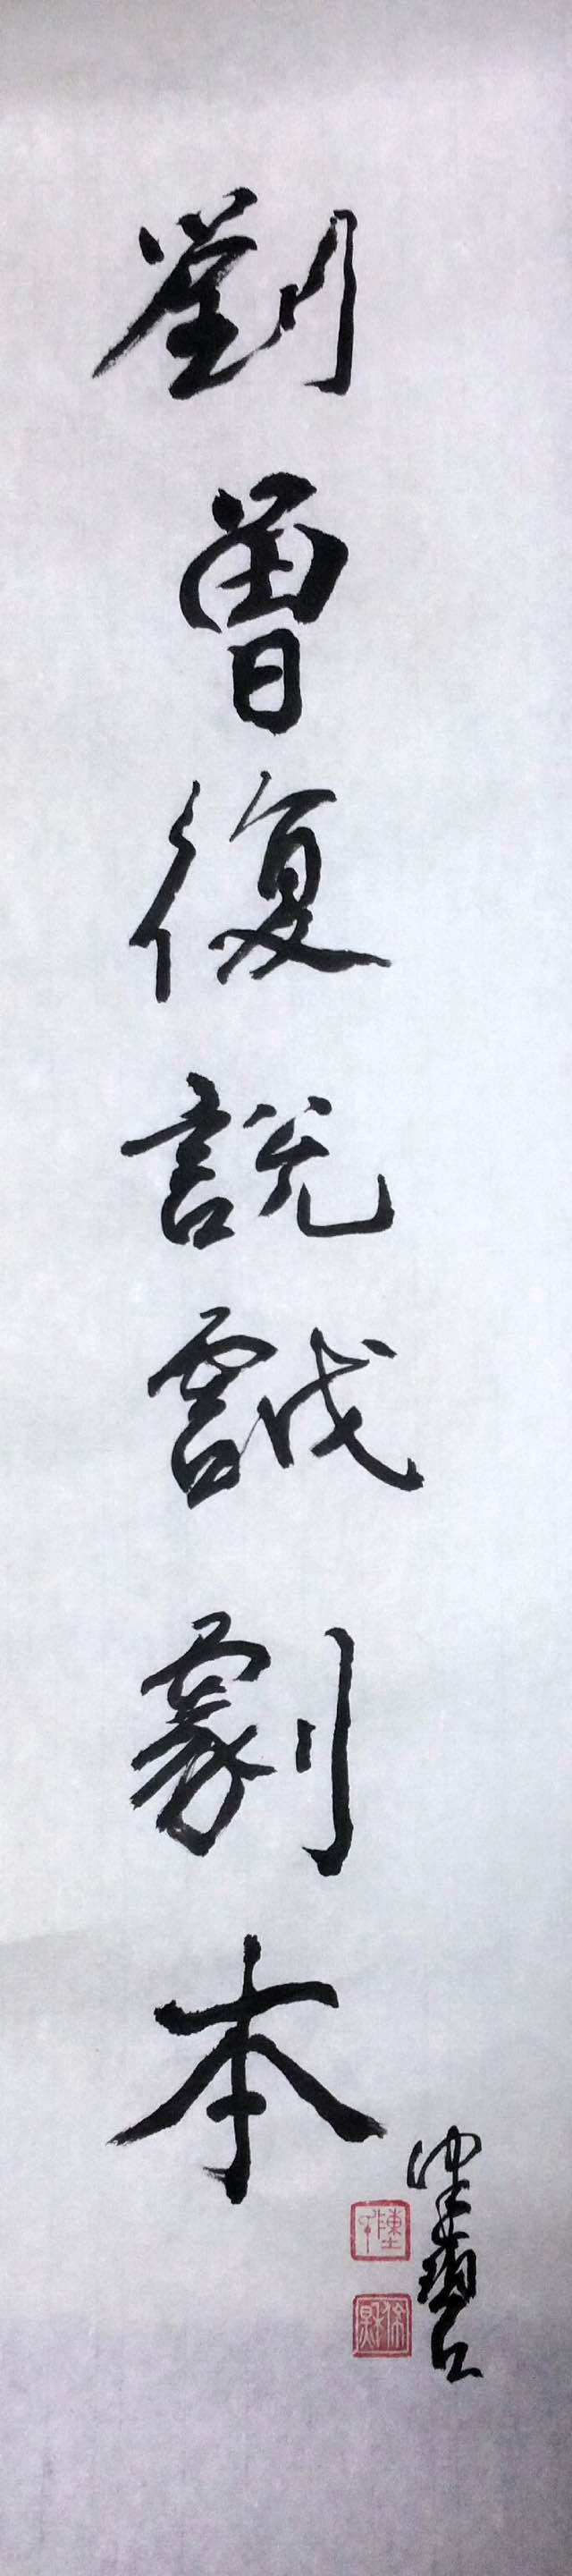
\includegraphics[height=1.30\textwidth,width=0.25\textwidth,viewport=0 0 620 2850,clip]{Figures_Peking-Opera/Liu_script-Inscription.JPG}
%\caption*{\hei 陈佩秋(谢稚柳~夫人)先生~题签}
\label{Chen-Peking_Opera_Script-Inscription-2015}
\end{figure}

\newpage
\pagestyle{empty}    % 清空页码                                      %
\begin{figure}[h!]
\centering
\vspace{+0.2in}
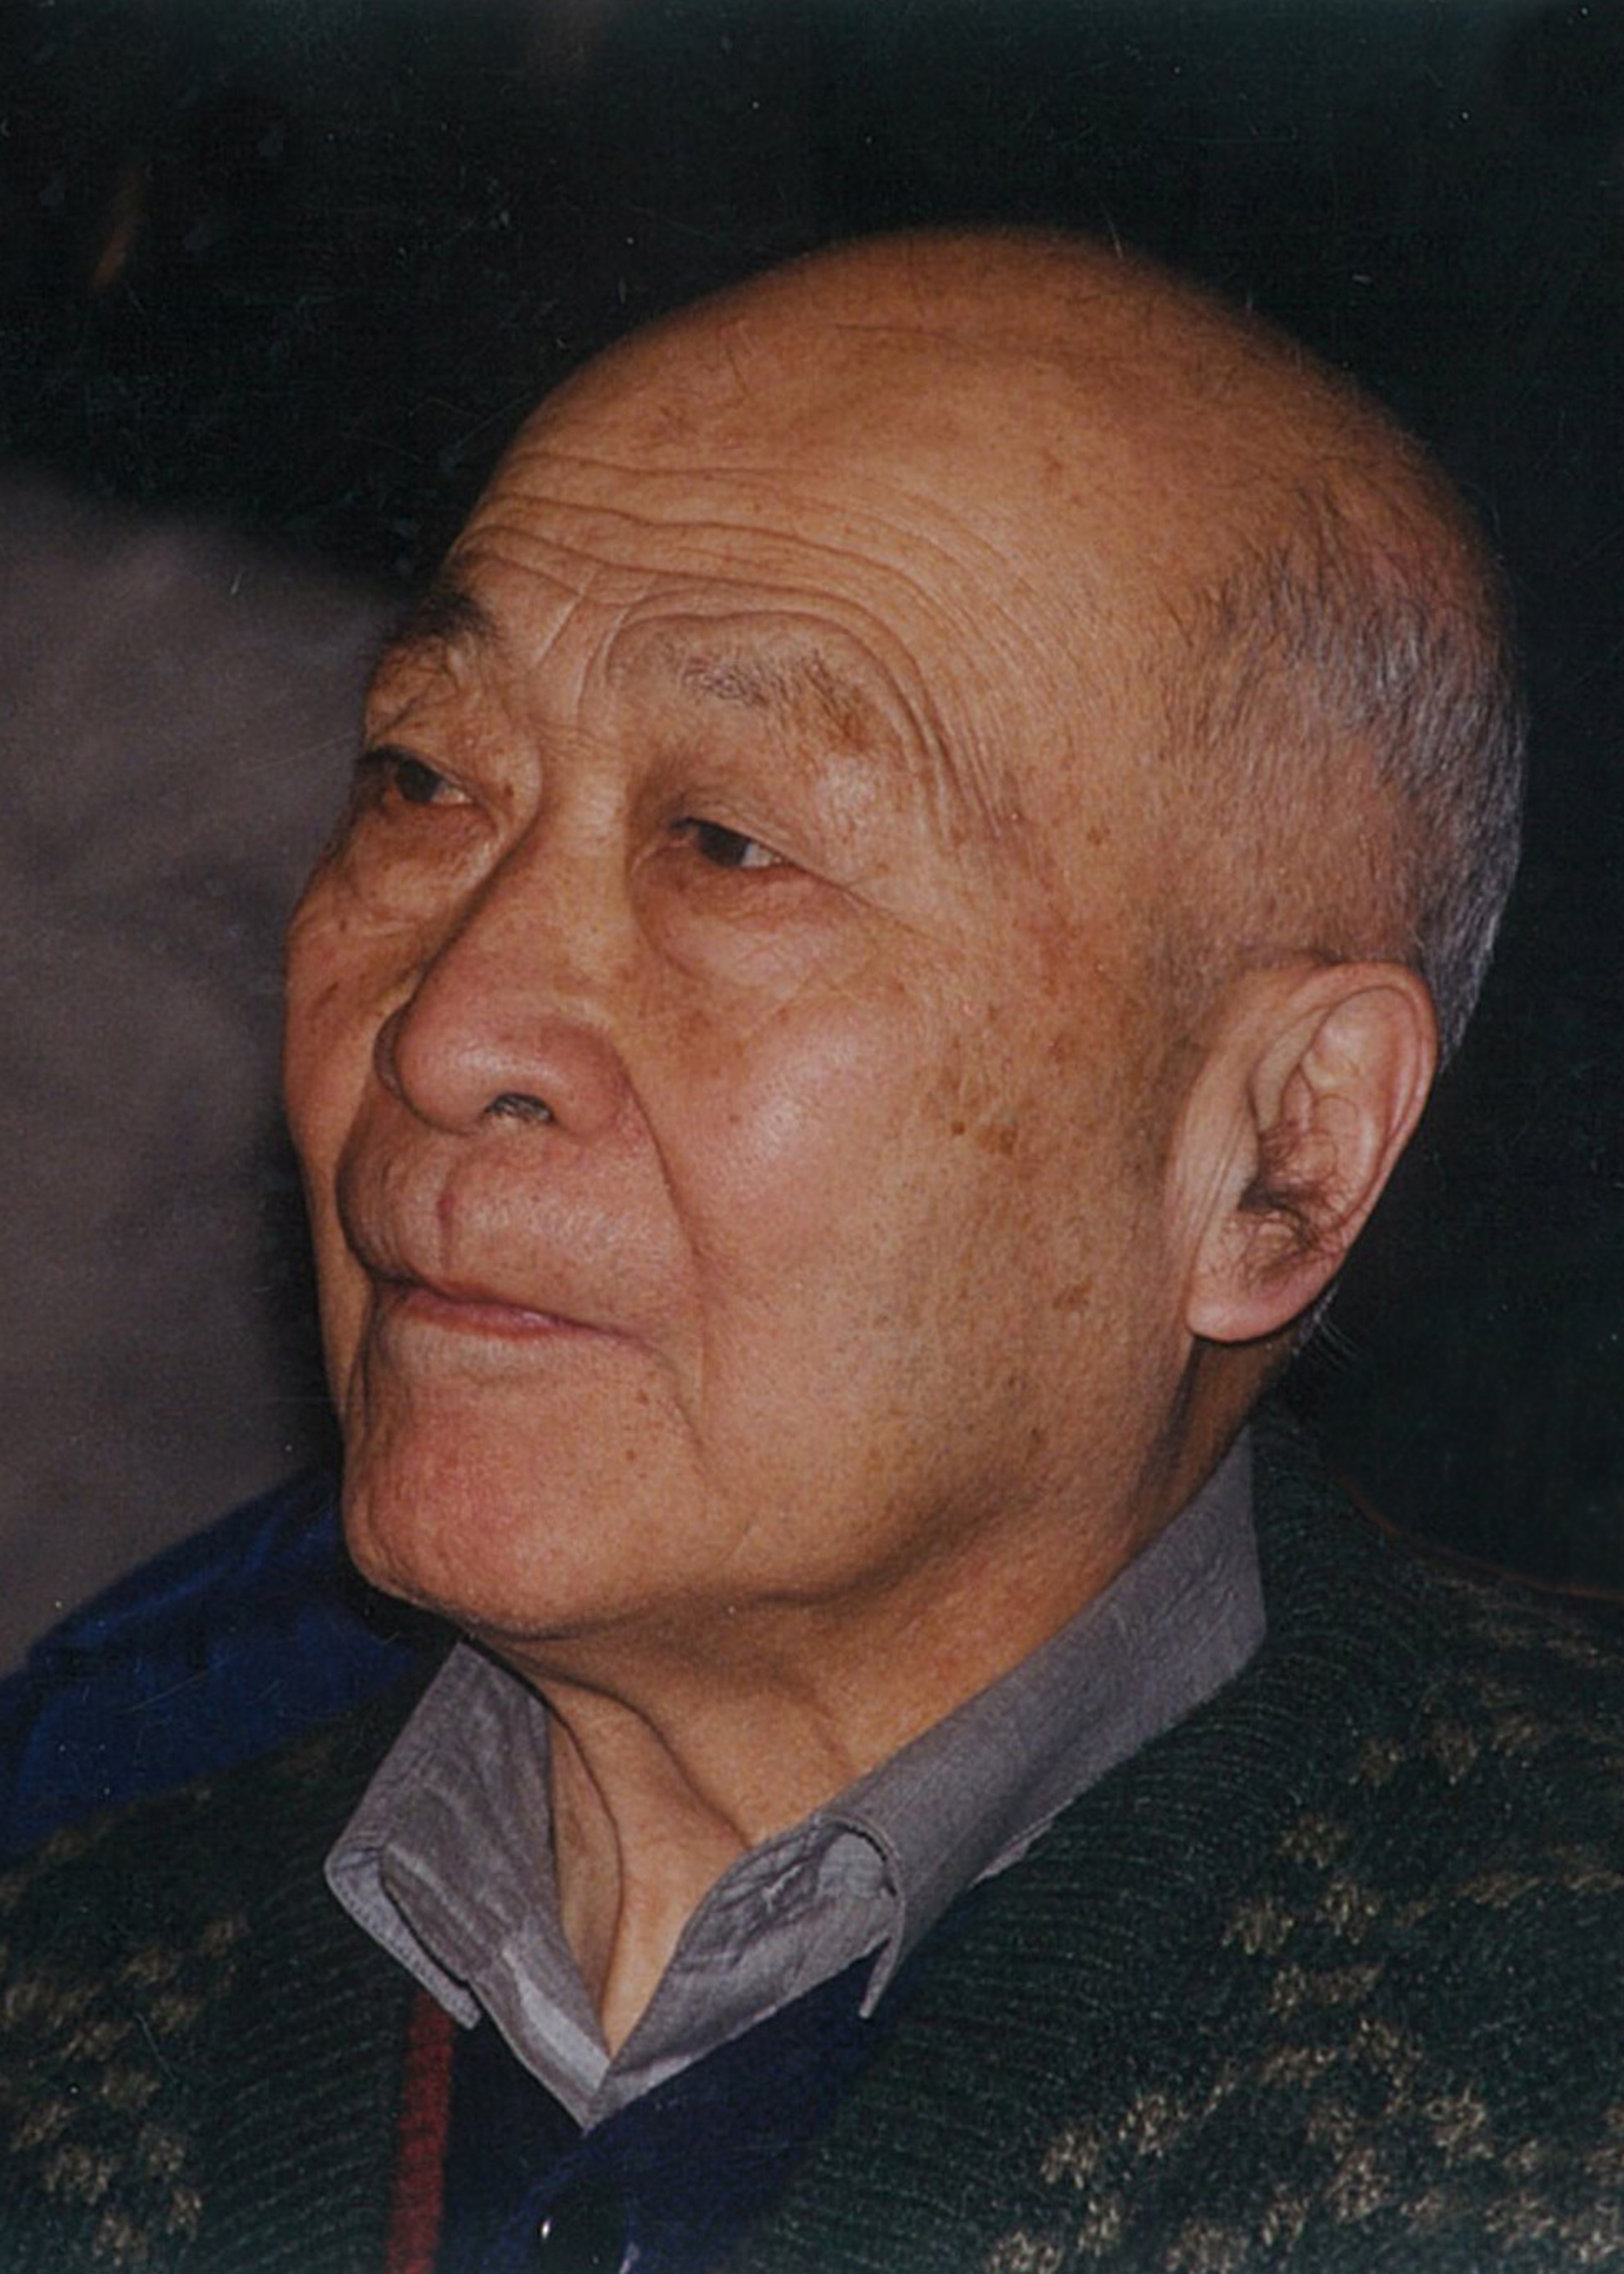
\includegraphics[height=1.20\textwidth,width=0.82\textwidth,viewport=0 0 360 520,clip]{Liu_Zengfu.jpg}
\caption*{\hei 刘曾复~教授~~(1914.11.9-2012.6.27)}
\label{Liu_Zengfu}
\end{figure}

\newpage
\begin{figure}[h!]
\centering
\vspace{-0.2in}
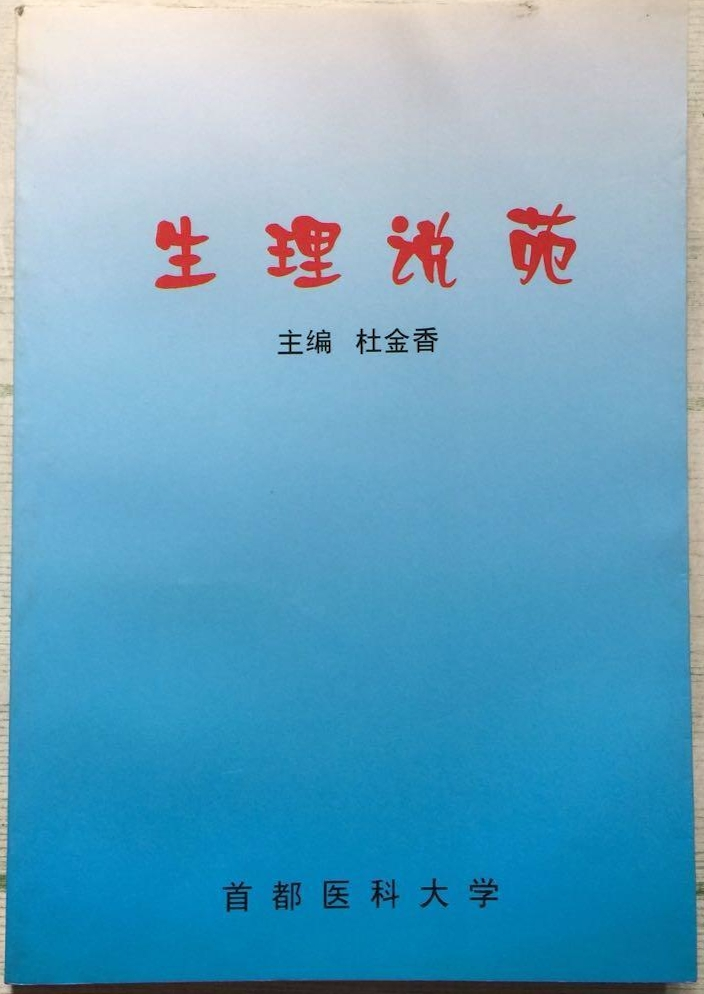
\includegraphics[height=0.65\textwidth,width=0.48\textwidth,viewport=0 0 700 1000,clip]{Liu-Physiology.jpg}
\label{Liu-Physiology}
\end{figure}
\begin{figure}[hbtp!]
\hspace*{-0.4in}
\begin{minipage}[t]{0.48\textwidth}
	\centering
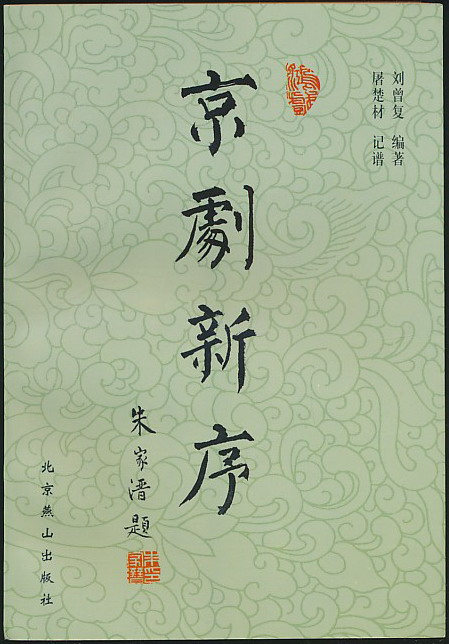
\includegraphics[height=1.50\textwidth,width=1.05\textwidth,viewport=0 0 450 650,clip]{Liu-Xinxu.jpg}
\end{minipage}
\hspace{0.3in}
\begin{minipage}[t]{0.48\textwidth}
	\centering
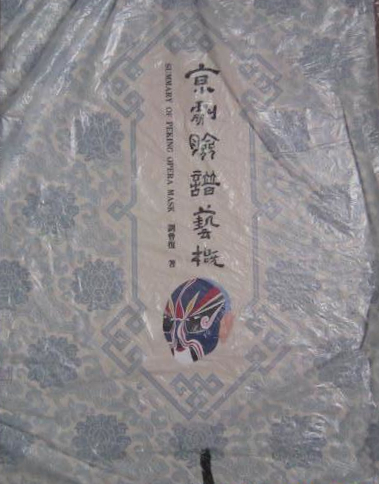
\includegraphics[height=1.50\textwidth,width=1.25\textwidth,viewport=0 0 410 490,clip]{Liu-Mask.jpg}
\end{minipage}
\vspace{1.0pt}
\caption*{\hei 刘曾复~教授~主要代表著作}
\label{Major_Works}
\end{figure}

\newpage
\begin{figure}[h!]
\centering
%\vspace{+0.2in}
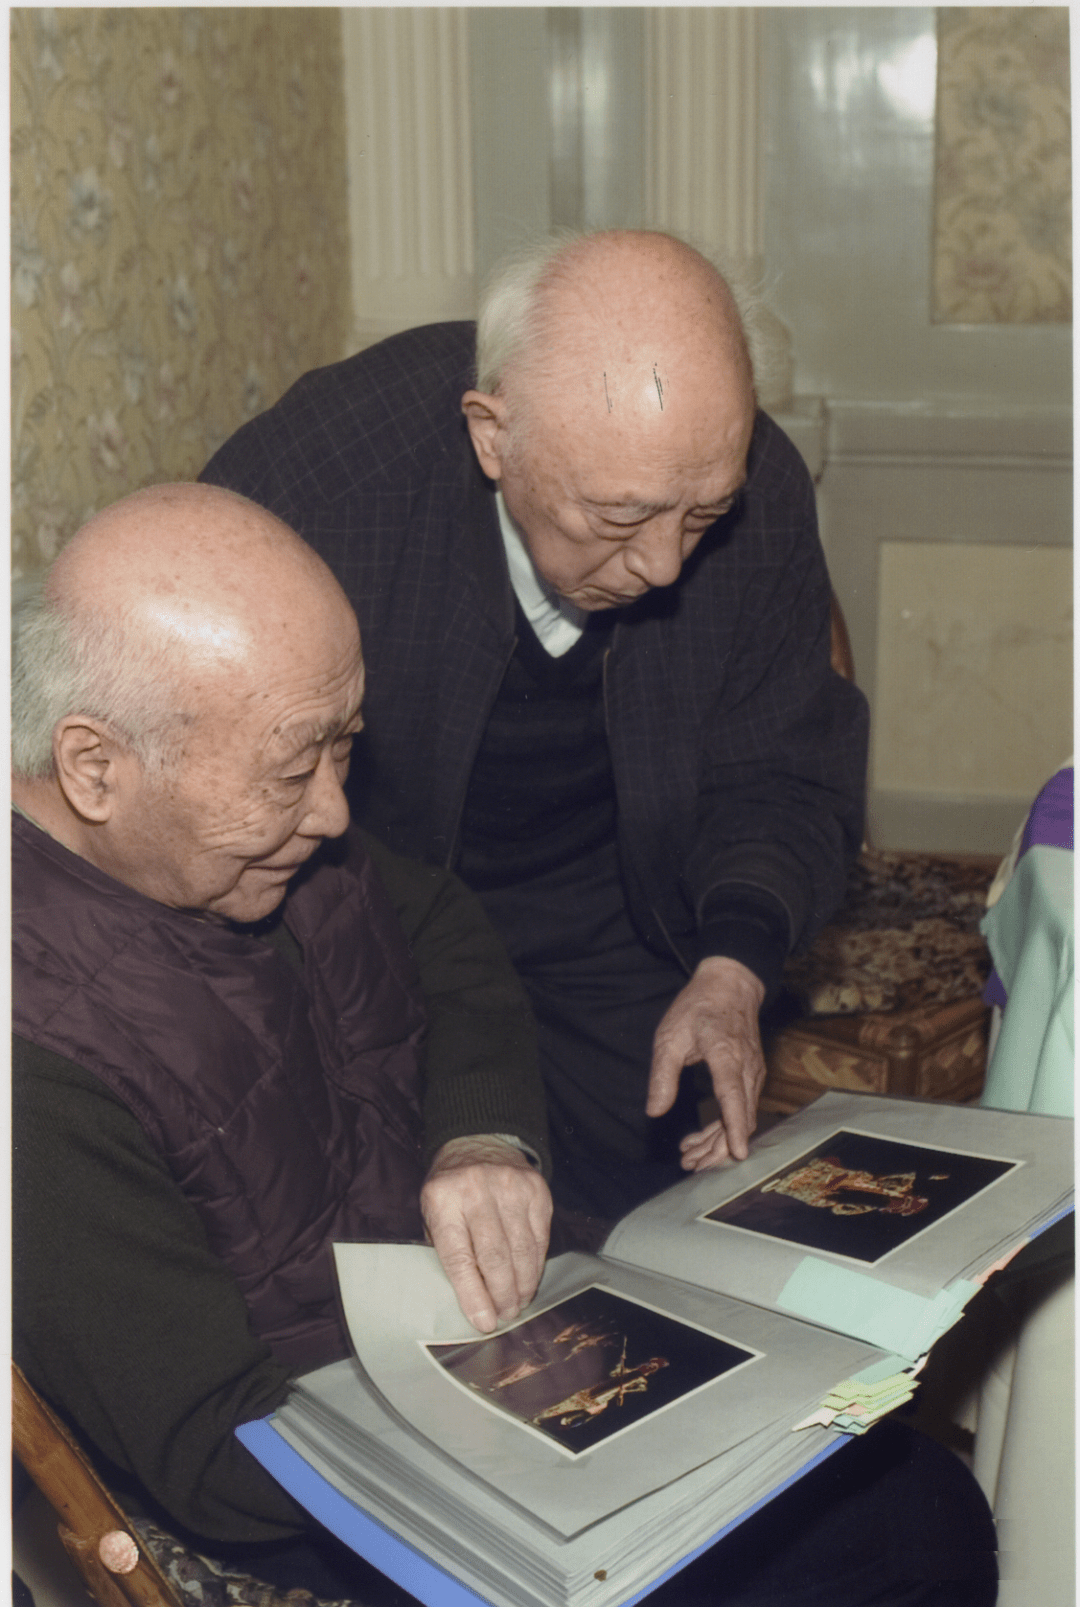
\includegraphics[height=1.38\textwidth,width=1.0\textwidth,viewport=0 0 1050 1550,clip]{Liu-Wu.png}
\caption*{\hei 刘曾复~先生~和~吴小如~先生}
\label{Collect_Liu_Wu}
\end{figure}

\newpage
\begin{figure}[h!]
\centering
%\vspace{-10.5pt}
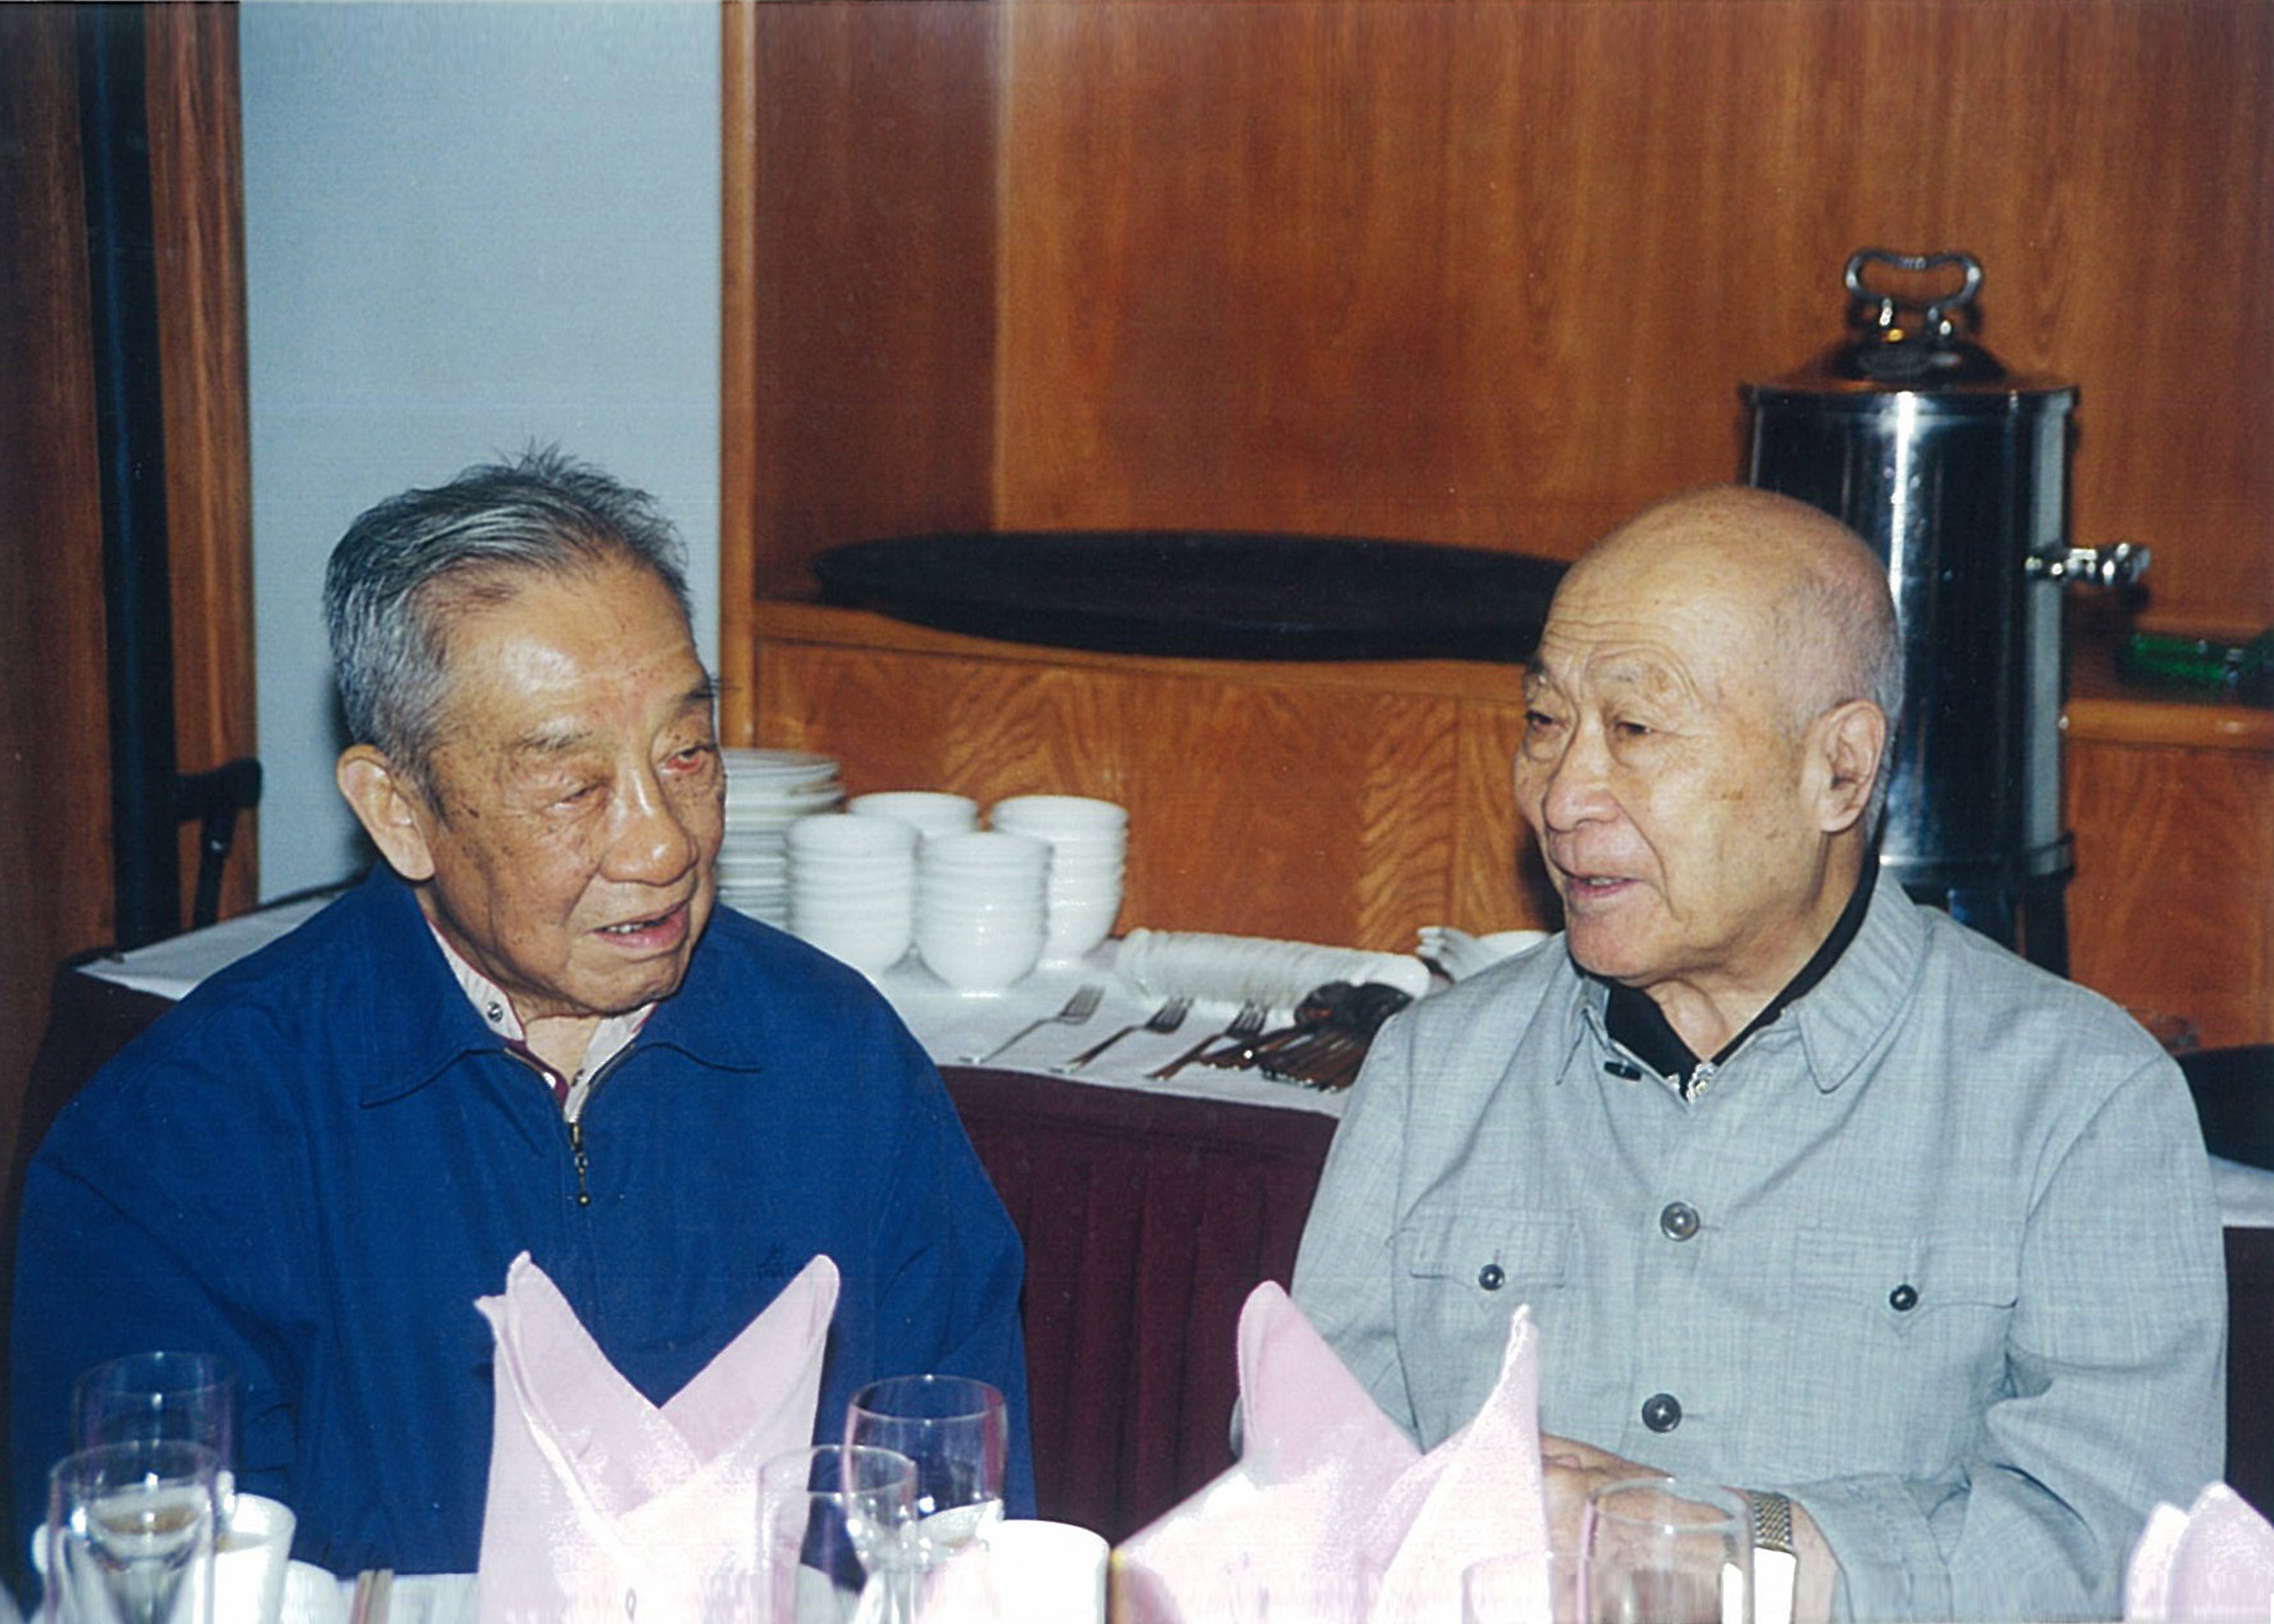
\includegraphics[height=0.60\textwidth,width=1.0\textwidth,viewport=0 0 500 300,clip]{Zhu-Liu.jpg}
\caption*{\hei 朱家溍~先生~和~刘曾复~先生}
\label{Collect_Zhu_Wu}
\end{figure}

\begin{figure}[h!]
\centering
%\vspace{-10.5pt}
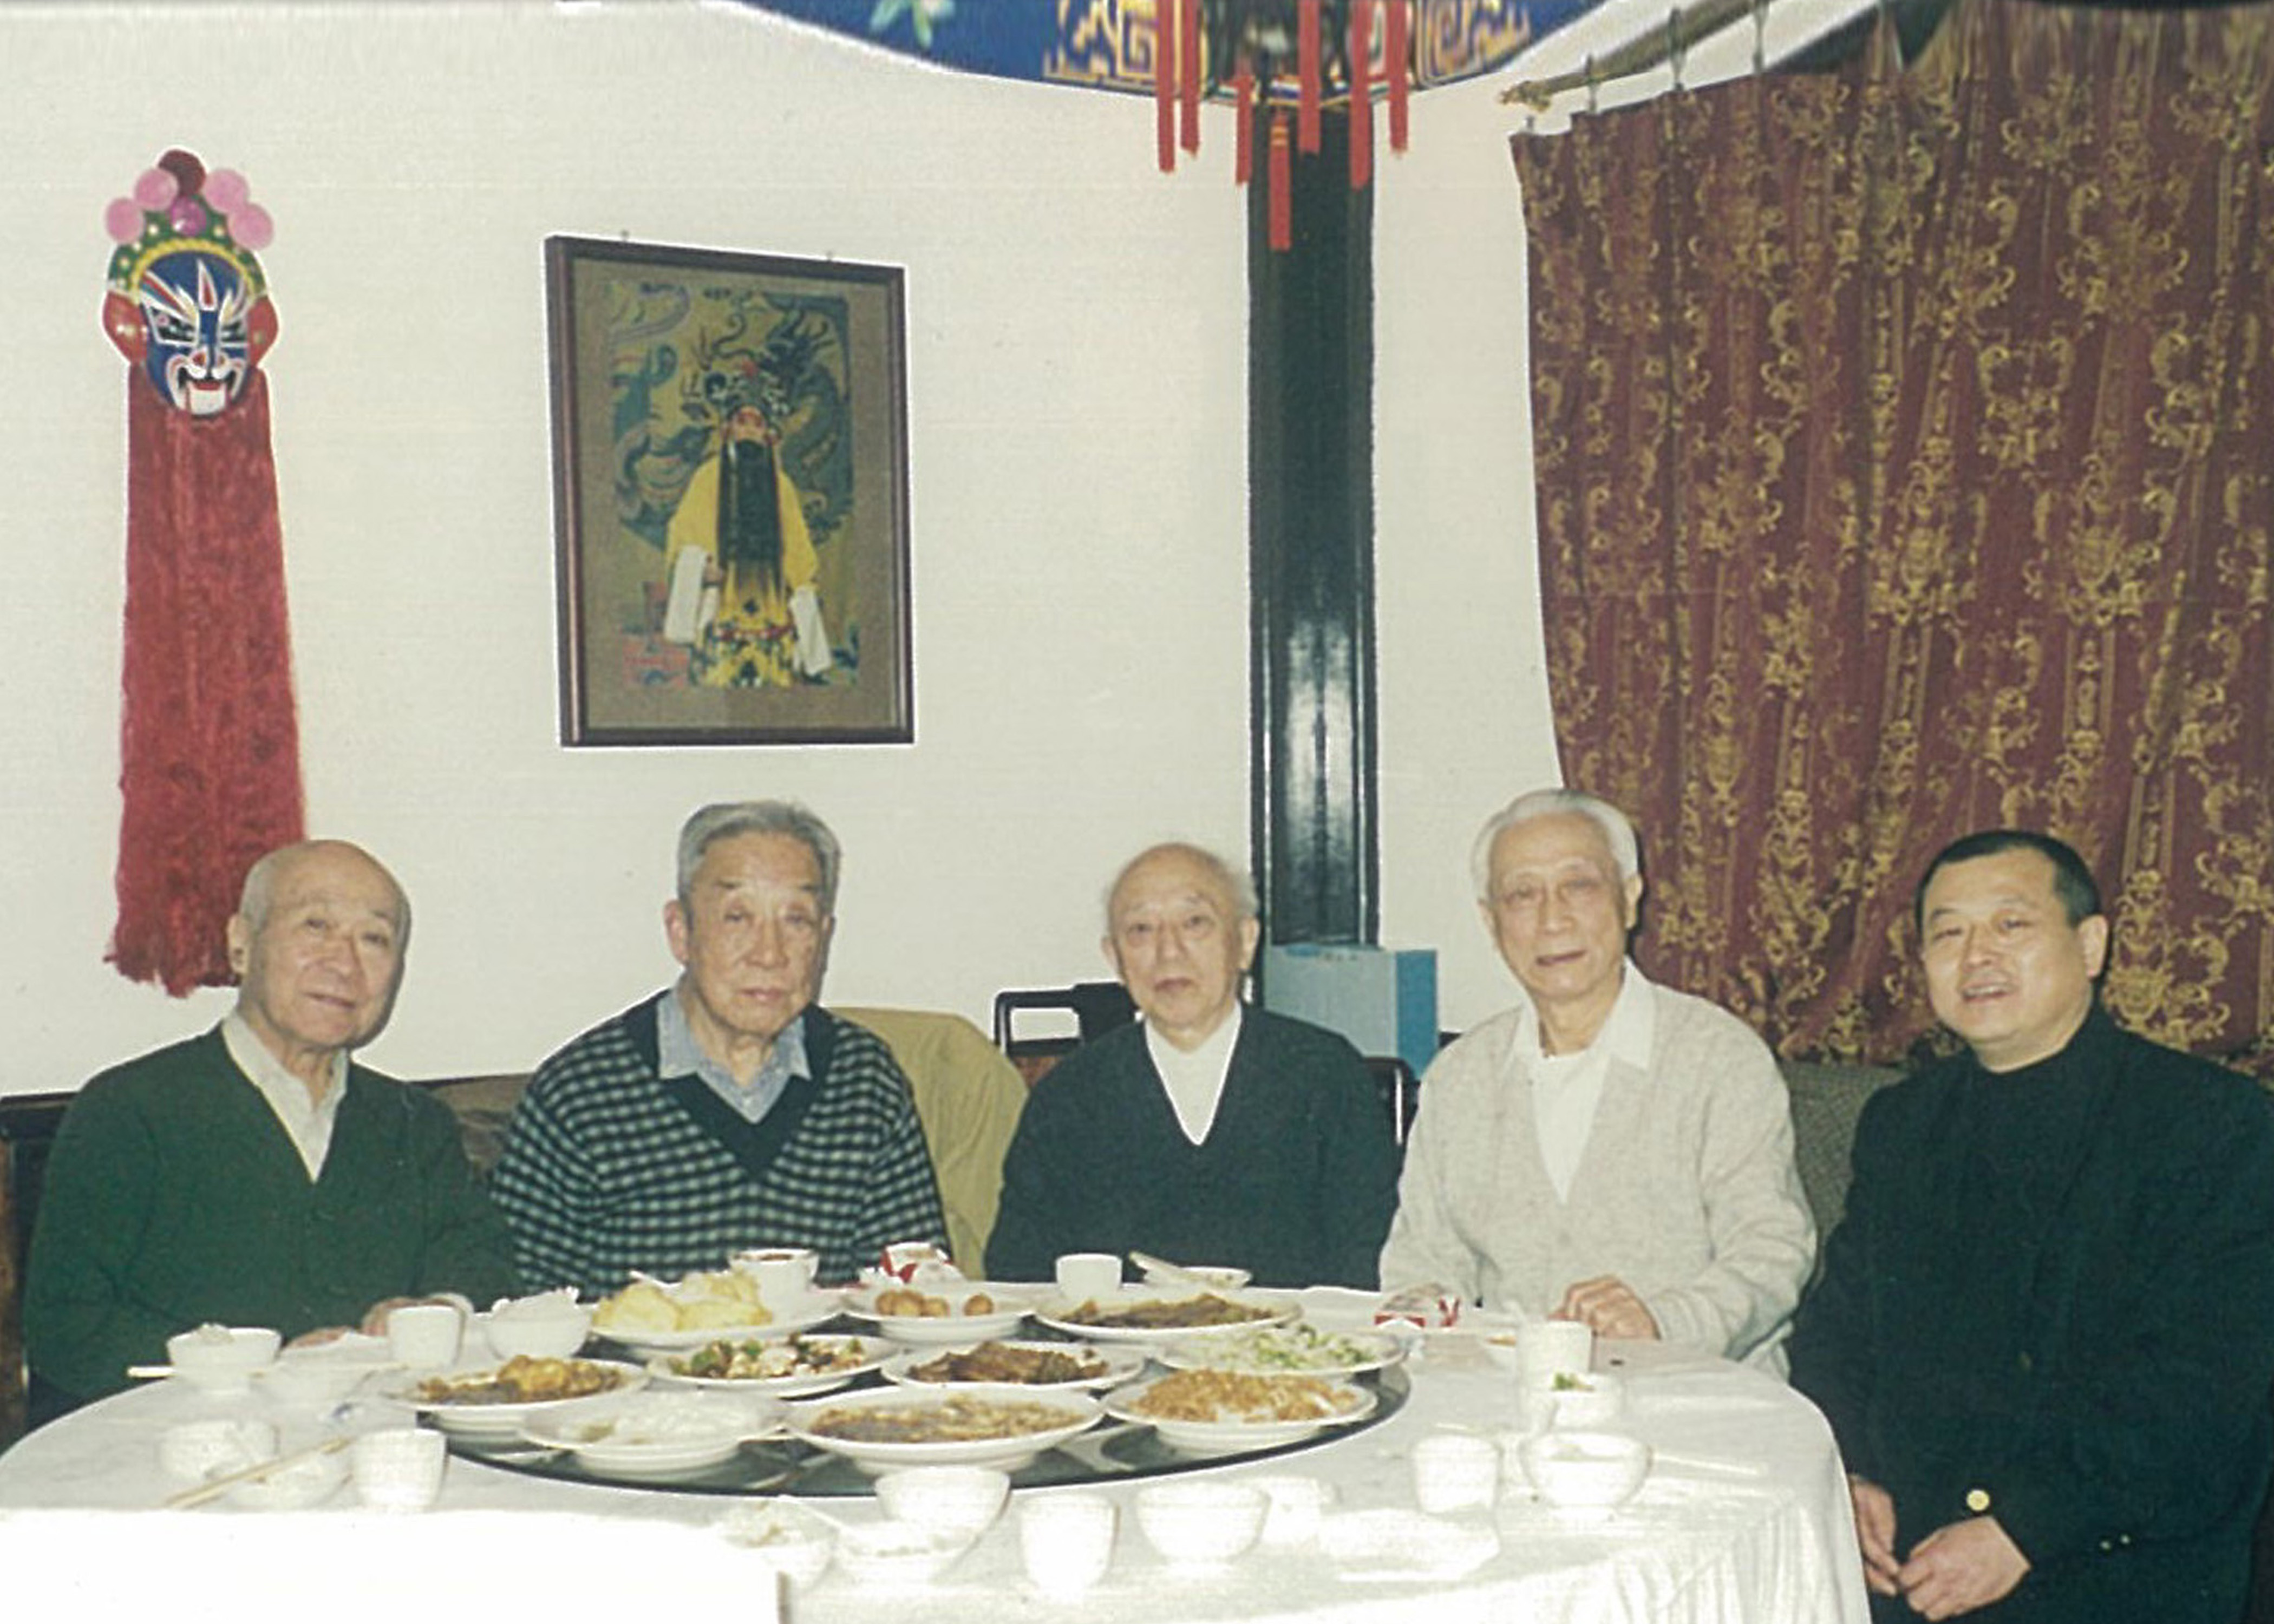
\includegraphics[height=0.60\textwidth,width=1.0\textwidth,viewport=0 0 500 300,clip]{Collect_Zhu-Liu-Wu-Wang.jpg}
\caption*{\hei 左起:~刘曾复~先生、朱家溍~先生、吴小如~先生、王金璐~先生~等~合影}
\label{Collect_Liy_Zhu_Wu_Wang}
\end{figure}

\newpage
\begin{figure}[h!]
\centering
\vspace{-0.6in}
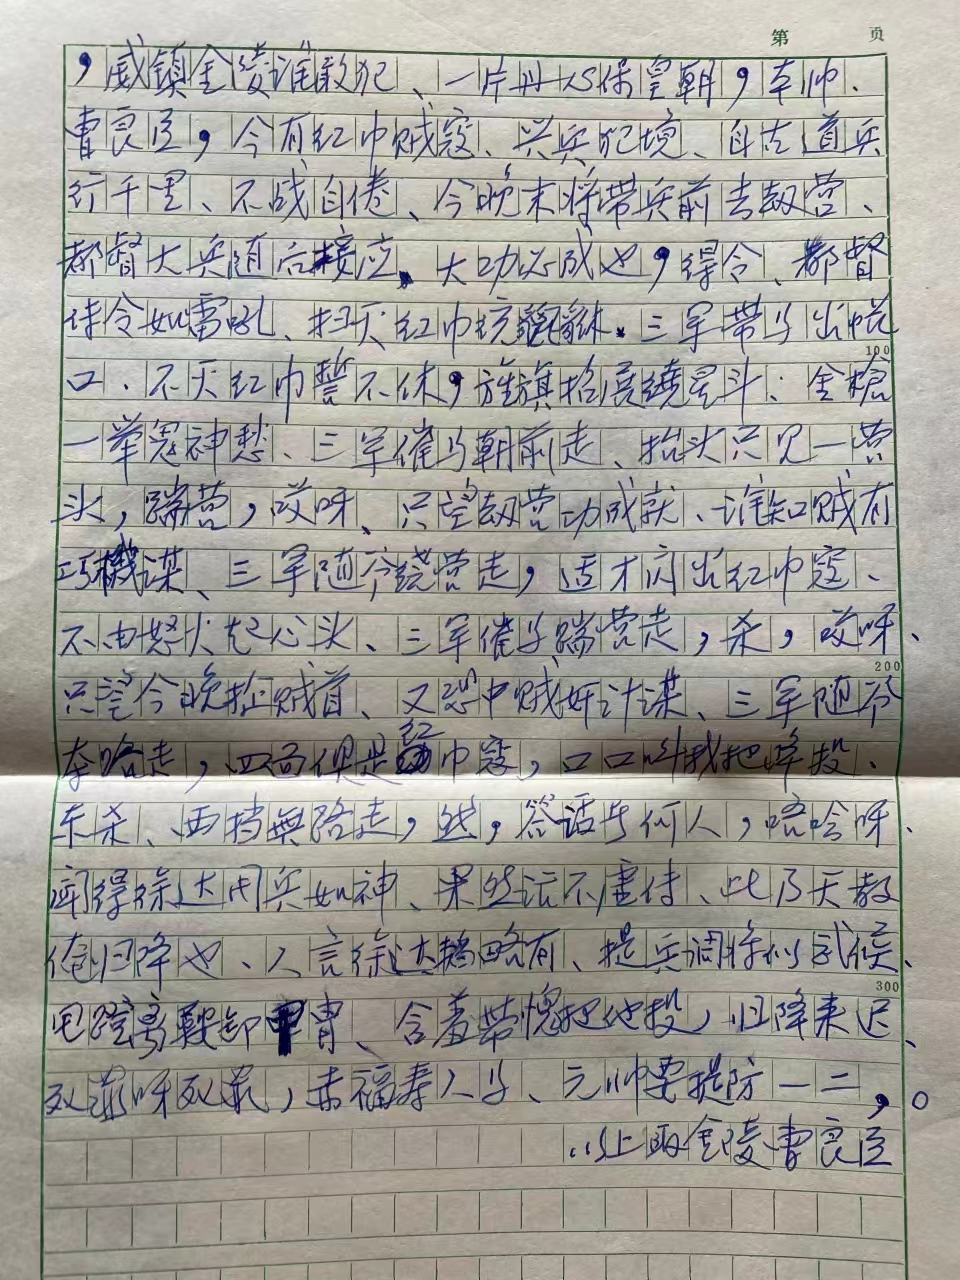
\includegraphics[height=0.68\textwidth,width=0.50\textwidth,viewport=0 0 950 1300,clip]{PekOpe_Liu-1.jpg}
\caption*{\hei 刘曾复~先生~抄录的《取金陵》曹良臣的单词}
\label{Liu-Script}
\end{figure}
\vspace{30pt}
\begin{figure}[hbtp!]
\hspace*{-0.5in}
\begin{minipage}[t]{0.53\textwidth}
	\centering
	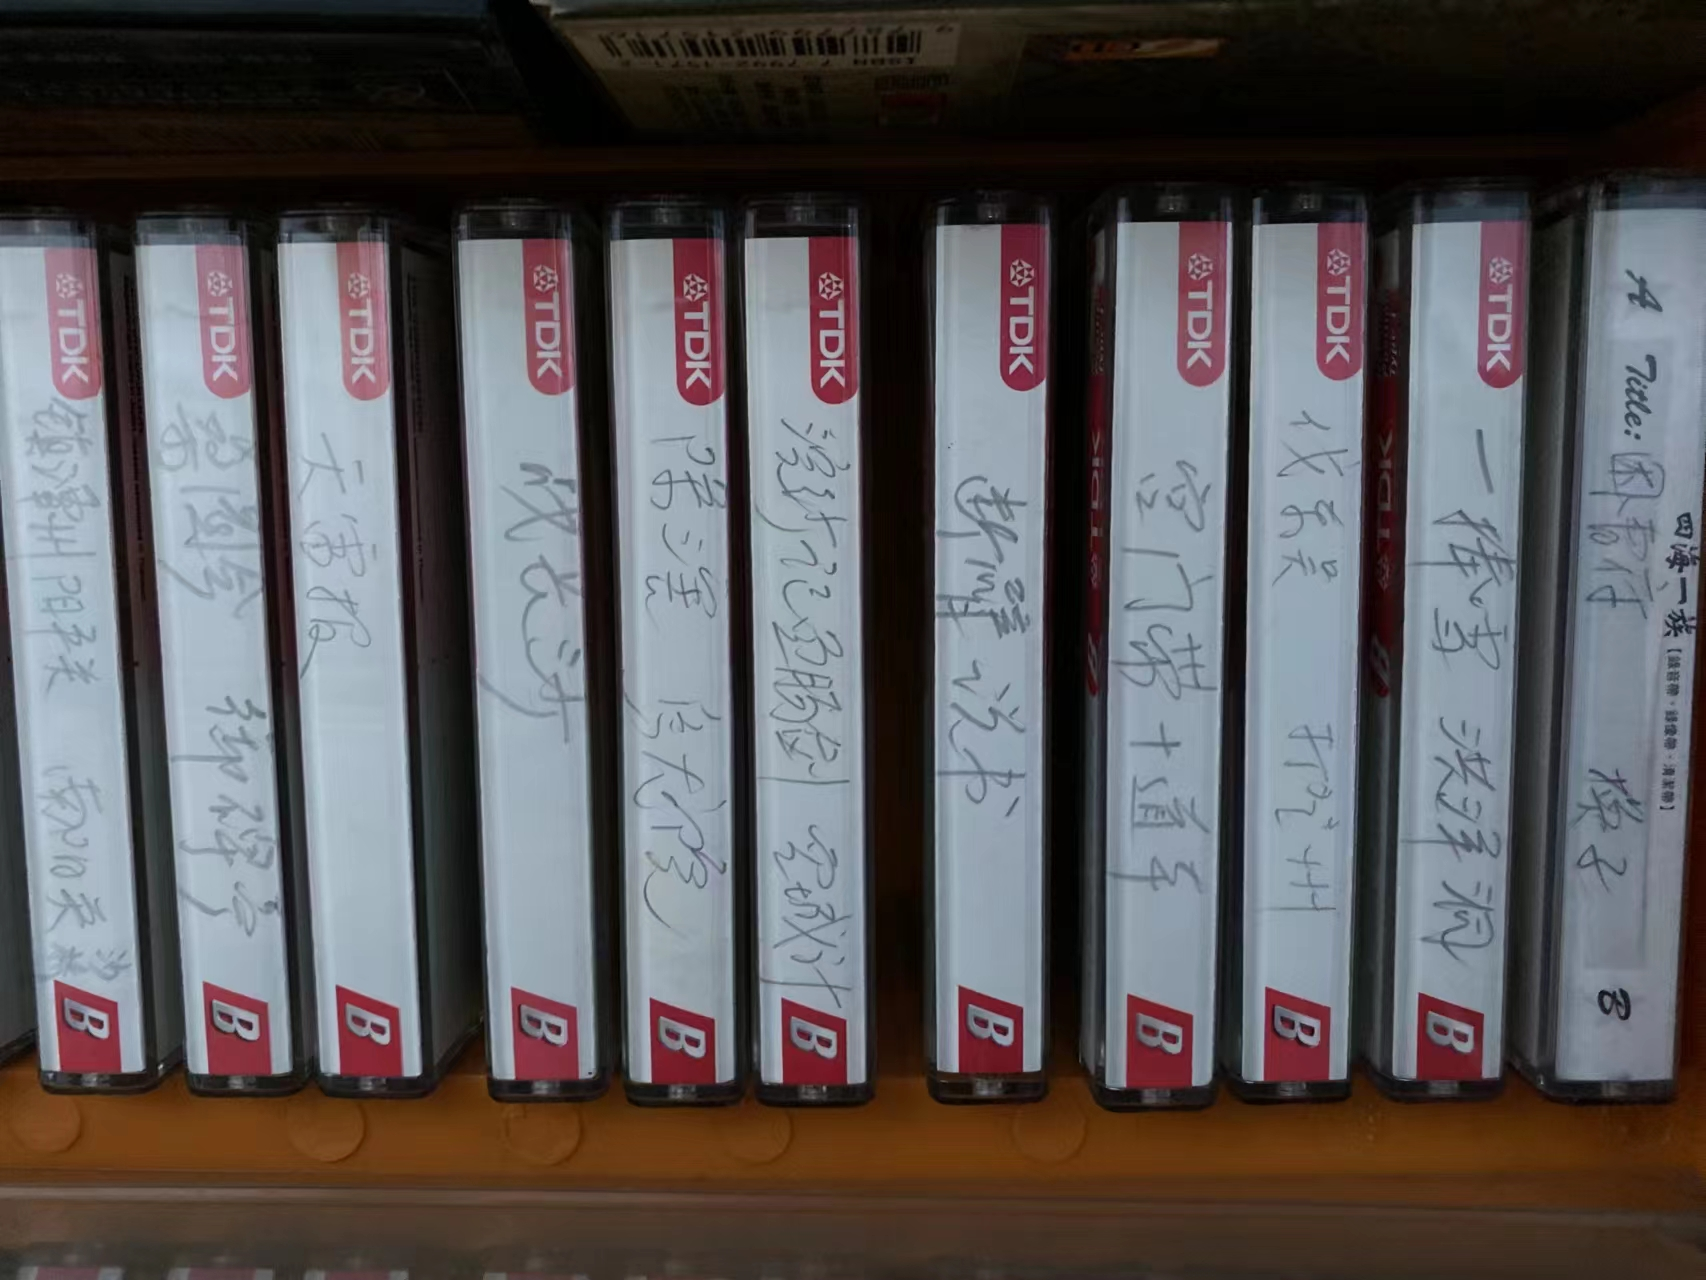
\includegraphics[height=1.00\textwidth,width=1.20\textwidth,viewport=0 0 1750 1300,clip]{PekOpe_Liu-2.jpg}
	\caption*{\hei \fontsize{8.5pt}{4.0pt}\selectfont{左:~刘曾复~先生~保存的部分说戏录音磁带}}
\end{minipage}
\hspace{0.6in}
\begin{minipage}[t]{0.43\textwidth}
	\centering
	\vspace{-3.7in}
	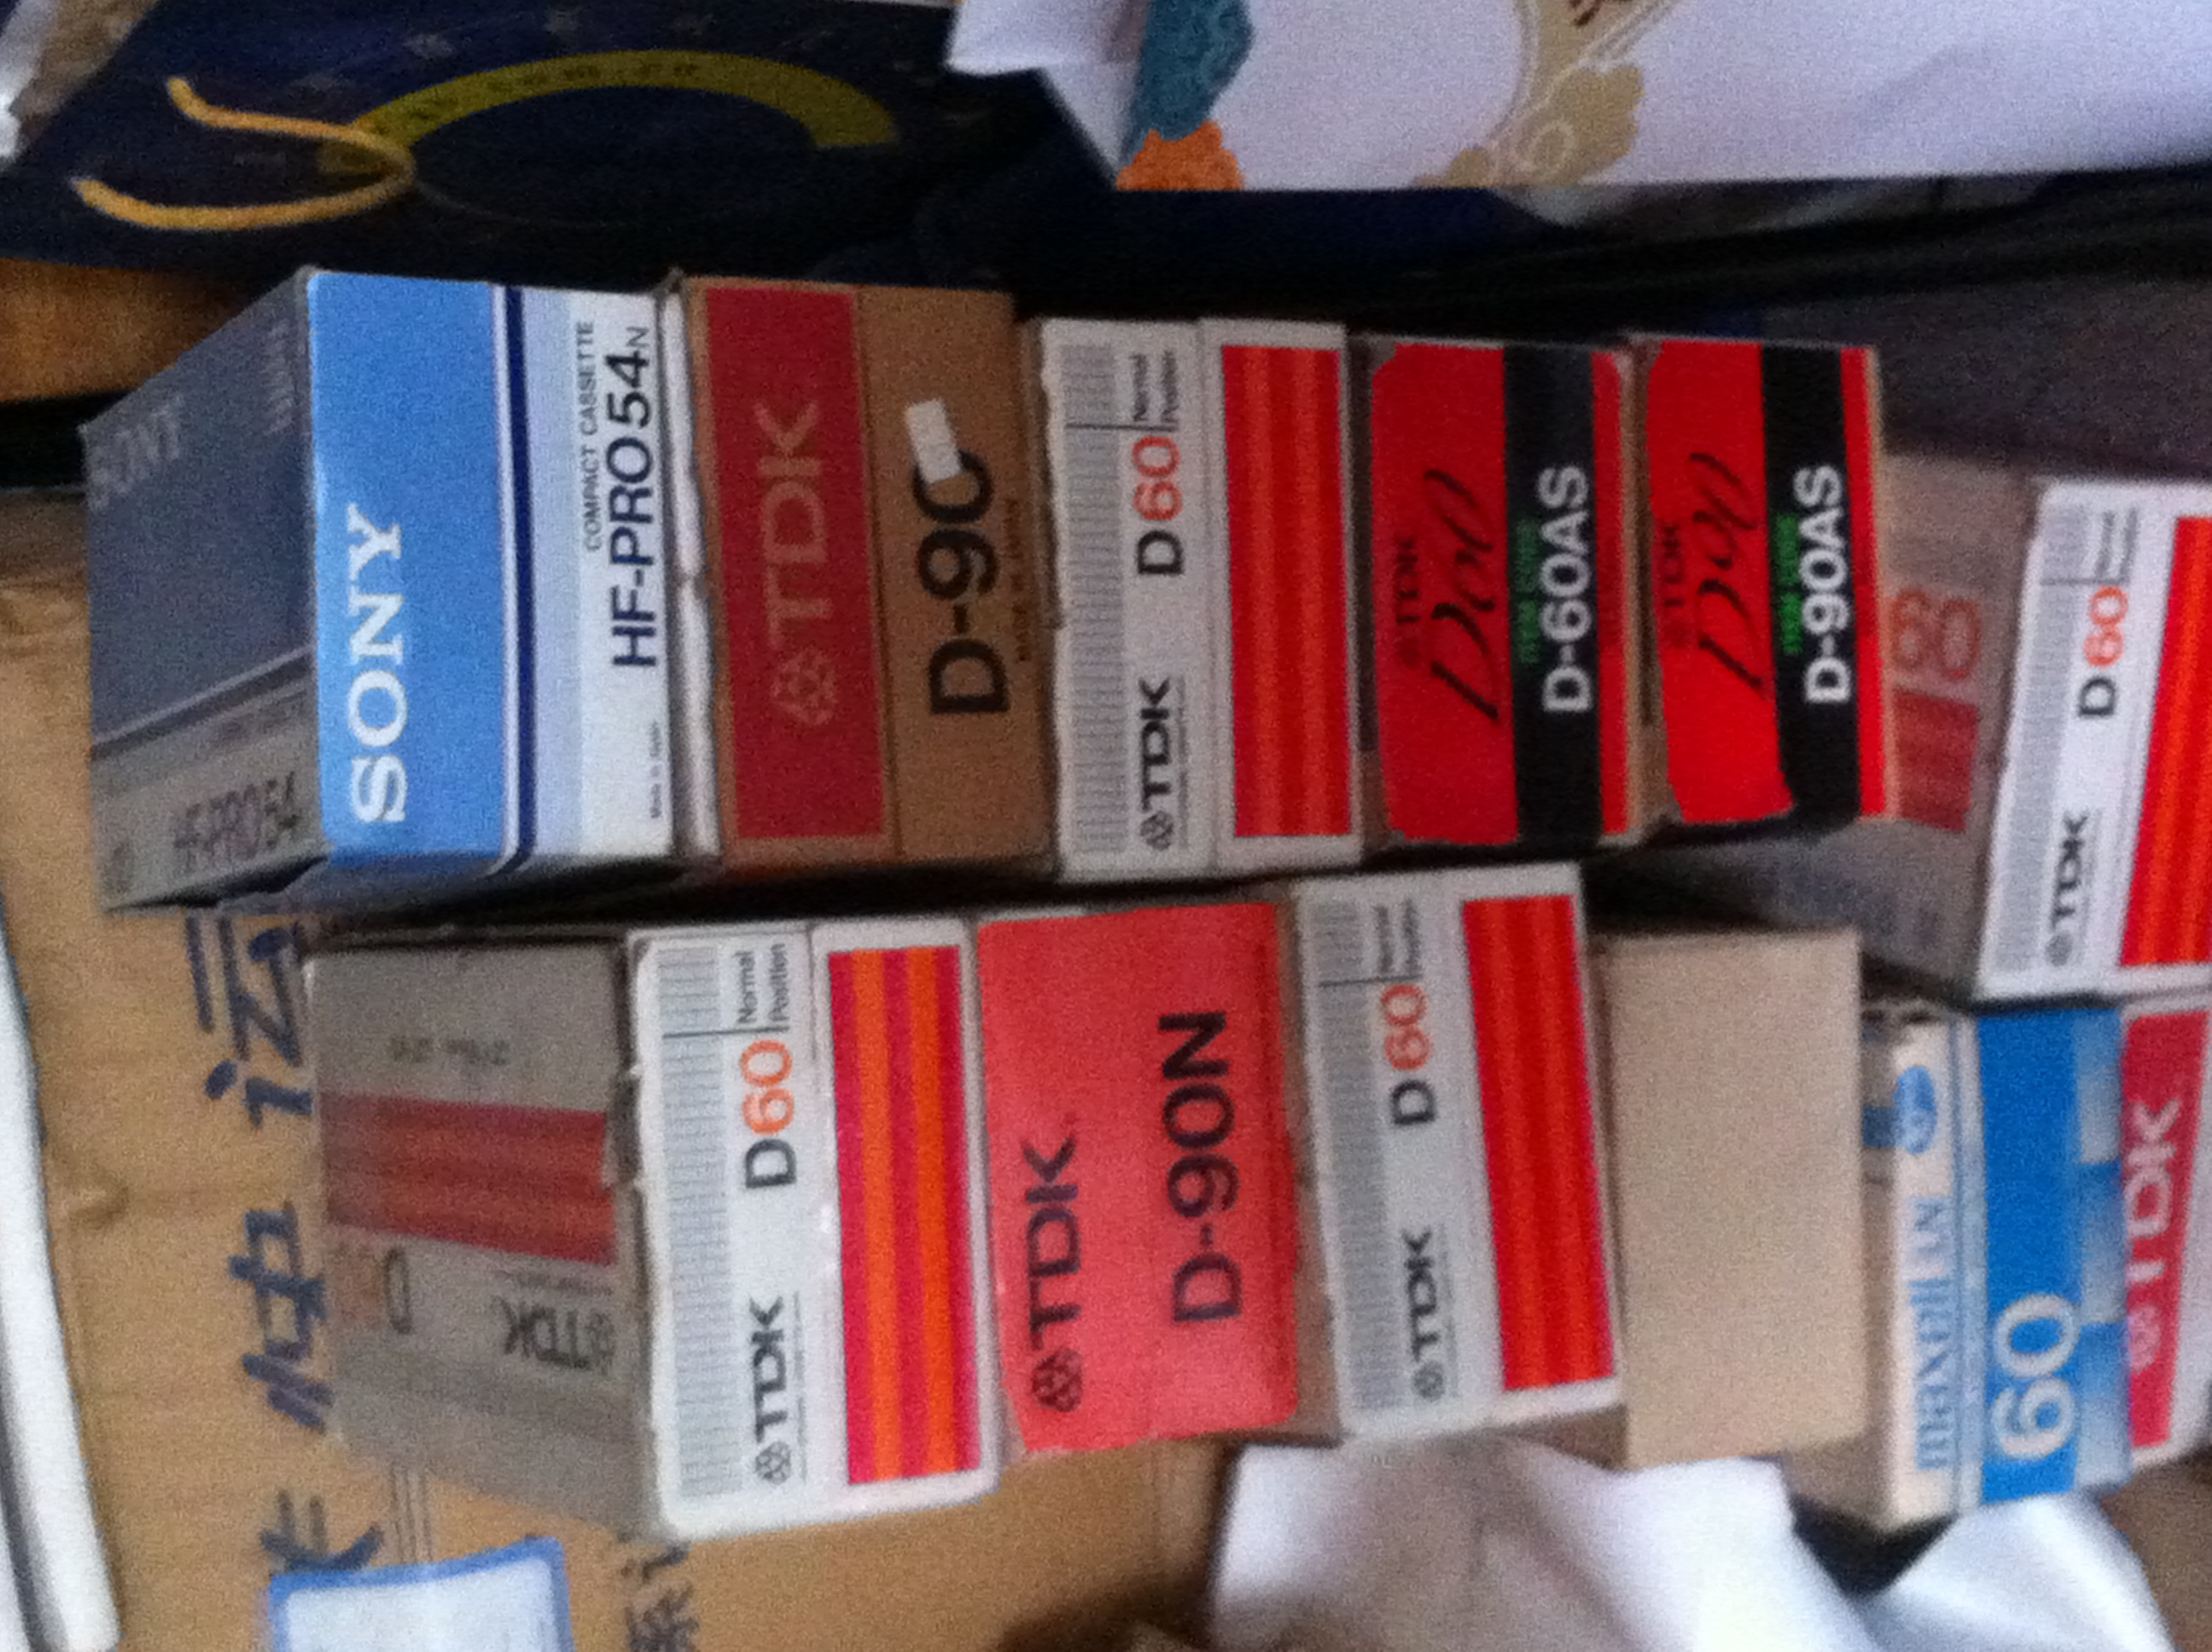
\includegraphics[height=1.10\textwidth,width=1.70\textwidth,angle=270, viewport=0 0 2750 1950,clip]{PekOpe_Wu-5.jpg}
%	\caption*{\hei \fontsize{8.5pt}{4.0pt}\selectfont{右:吴小如~先生~保存的刘曾复先生的说戏录音磁带}}
	\caption*{\hei \fontsize{8.5pt}{4.0pt}\selectfont{右:吴小如~先生~保存的各类说戏录音磁带}}
\end{minipage}
\label{Records}
\end{figure}
\newpage
\begin{figure}[h!]
\centering
\vspace{-0.6in}
	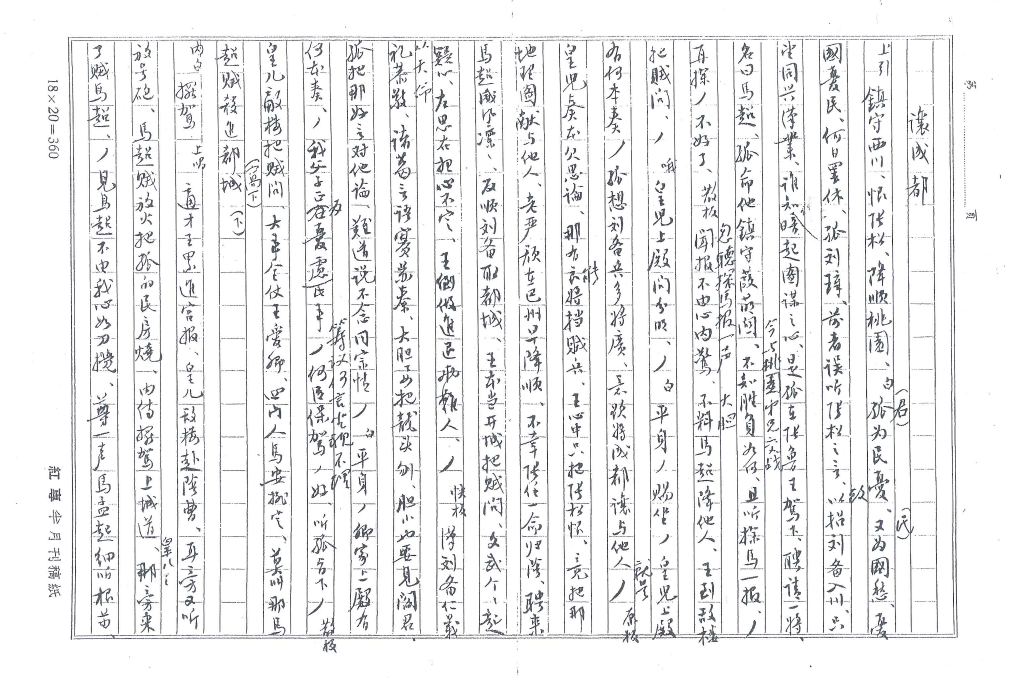
\includegraphics[height=0.50\textwidth,width=0.78\textwidth,viewport=0 0 750 470,clip]{PekOpe_Wu-script-1.png}
	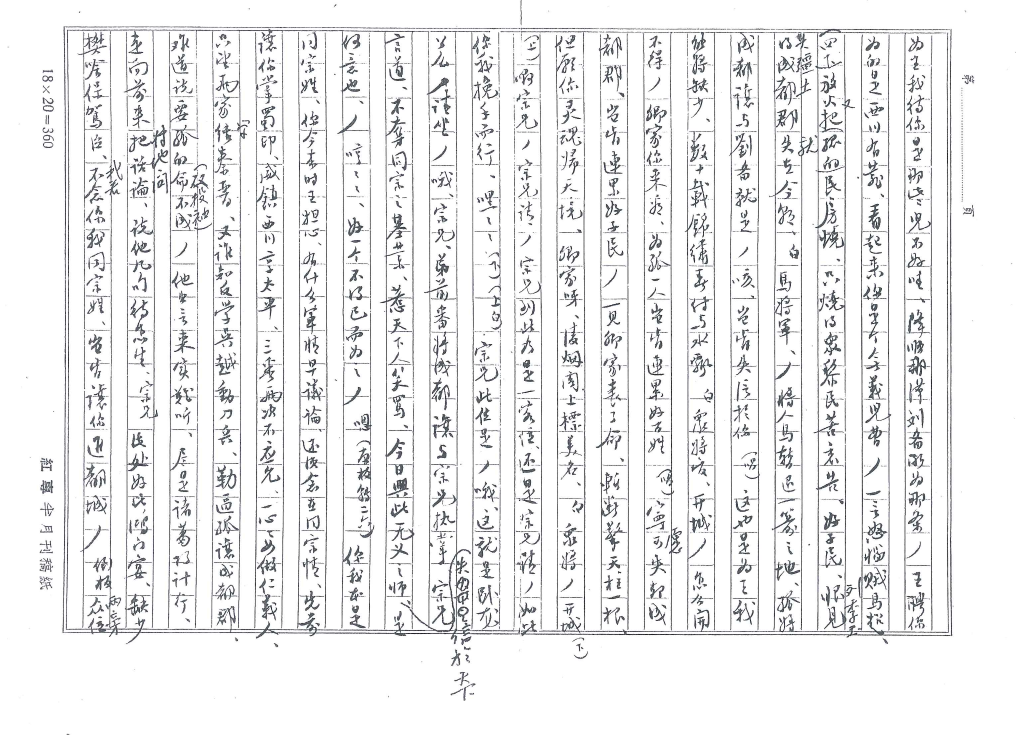
\includegraphics[height=0.50\textwidth,width=0.81\textwidth,viewport=0 0 750 520,clip]{PekOpe_Wu-script-2.png}
	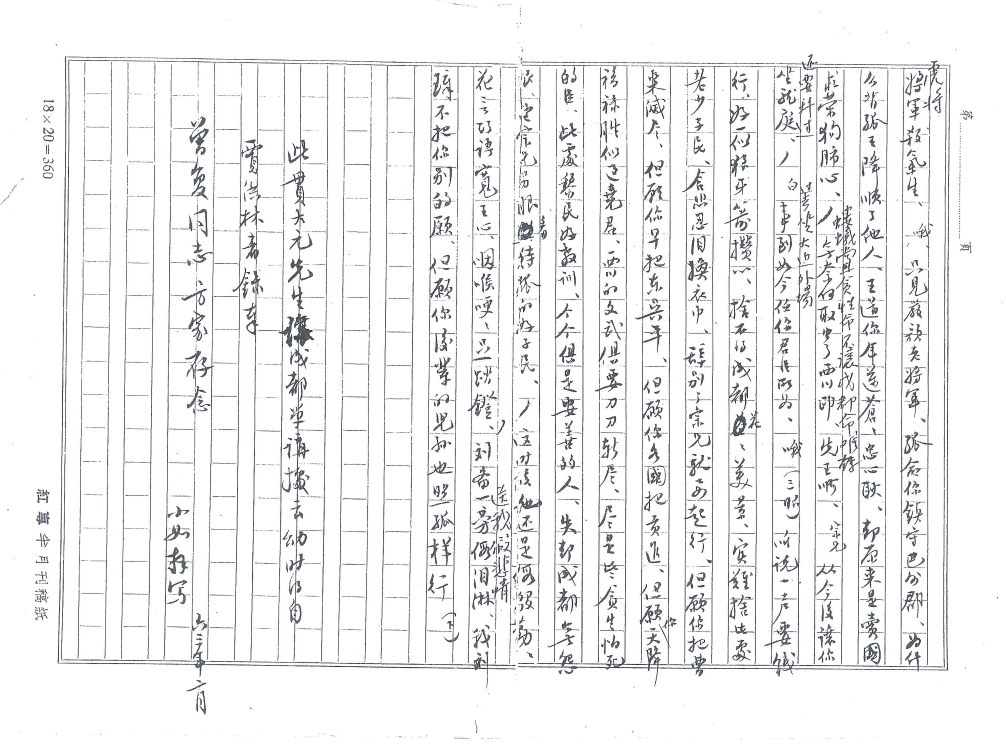
\includegraphics[height=0.50\textwidth,width=0.8\textwidth,viewport=0 0 750 500,clip]{PekOpe_Wu-script-3.png}
%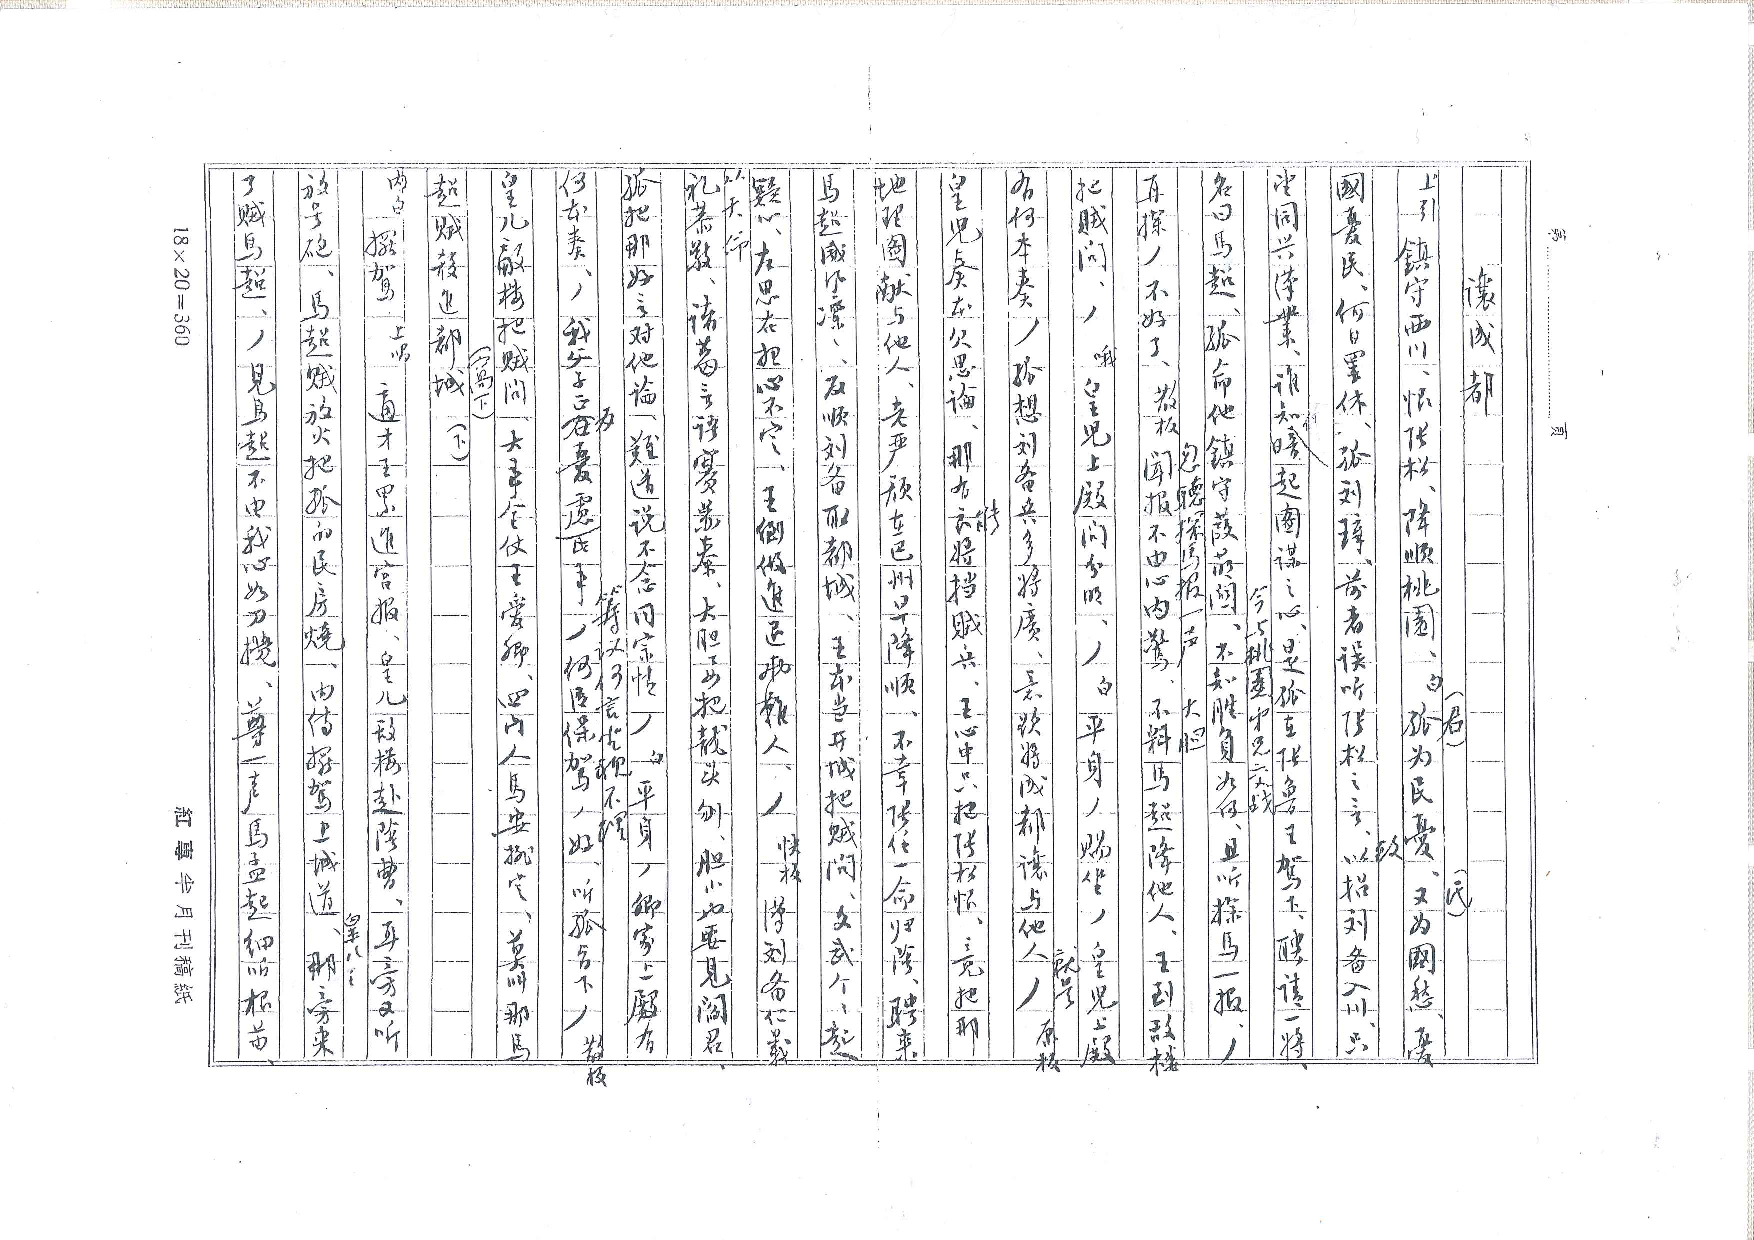
\includepdf[fitpaper]{PekOpe_Wu-script.pdf}
\caption*{\hei 吴小如~先生~抄录的~《让成都》刘璋的单词(贯大元~先生~传)复印件,刘曾复~先生~作了修改}
\label{Wu-Script}
\end{figure}

\newpage
\begin{figure}[h!]
\centering
%\vspace{-10.5pt}
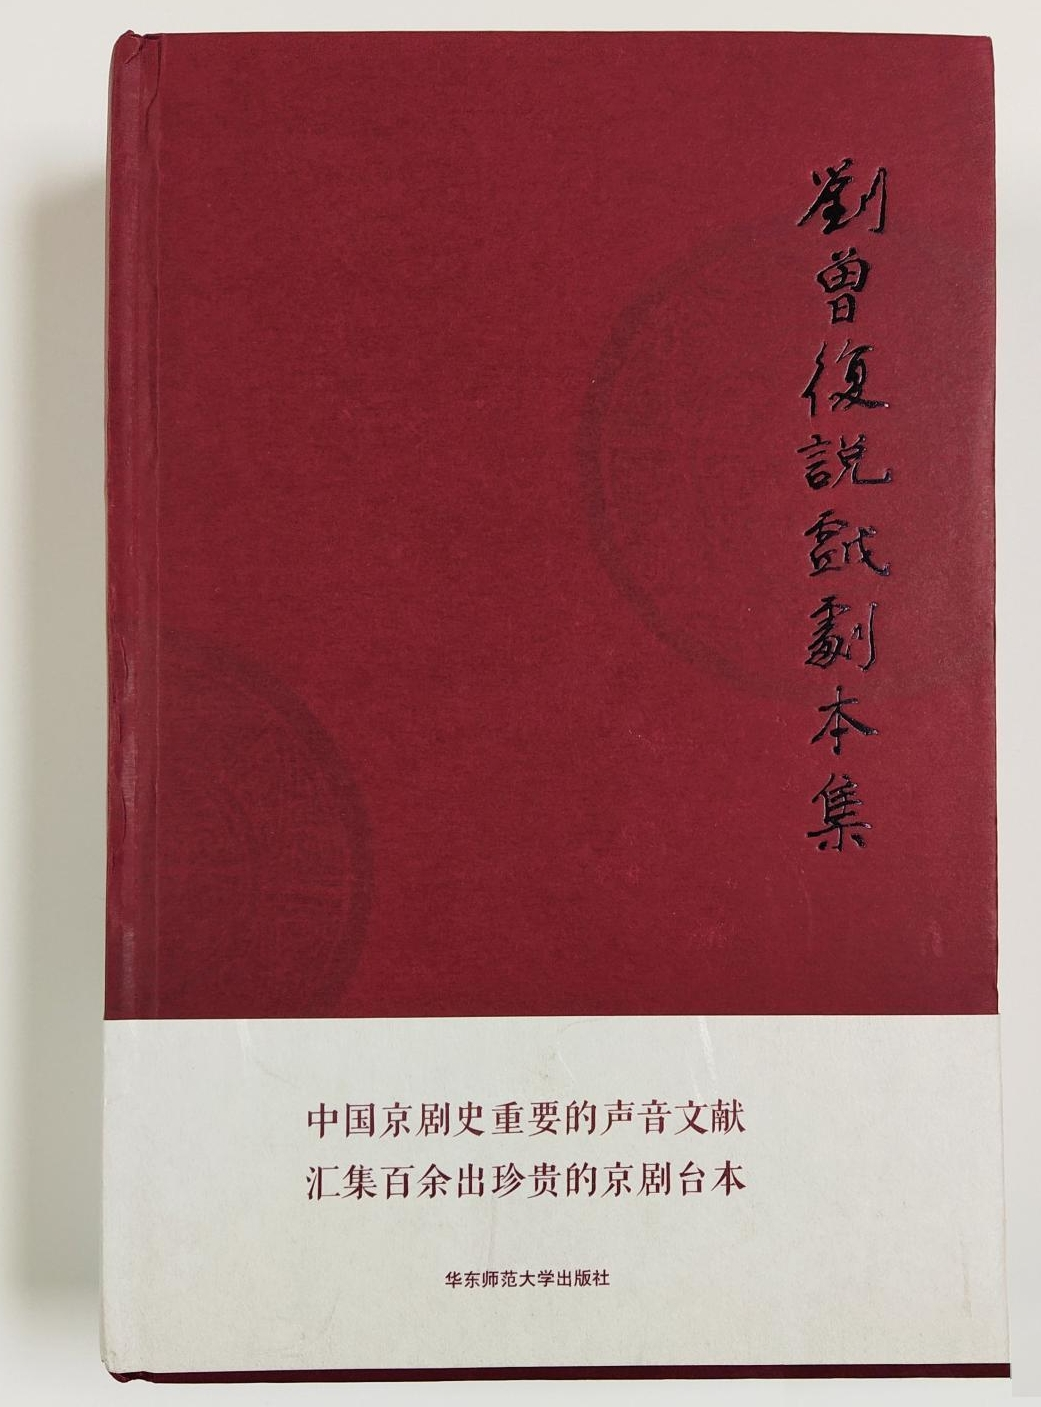
\includegraphics[height=1.30\textwidth,width=1.02\textwidth,viewport=0 0 1030 1400,clip]{Figures_Peking-Opera/Liu_script.jpg}
\caption*{\hei \fontsize{8.5pt}{4.0pt}\selectfont{《刘曾复说戏剧本集》初版~(上海~华东师范大学出版社~2015.08)~书影}}
\label{Peking_Opera_Script}
\end{figure}
%\keywords{Keyword1; Keyword2; Keyword3}


%%\newpage
\newpage
\phantomsection %实现目录的正确跳转
\setcounter{page}{0}
\pagenumbering{roman}
%\hypertarget{ux8bf4-ux660e}{
\addcontentsline{toc}{section}{\hei 说~~~~~~明}
	\section*{\hei \large 说\hspace{35pt}明}\label{ux8bf4-ux660e}%}
\pagestyle{fancy}    %与文献引用超链接style有冲突
\chead{说~明} % 页眉中间位置内容

\setlength{\parindent}{24pt}{     %
	此为个人整理的刘曾复教授说戏录音的文本稿,\textbf{主要根据刘曾复先生为中国戏曲学院提供的百余出说戏录音为底本,并结合刘曾老在其余场合的说戏录音}\upcite{Liu-Shuoxi-Record}%\textsuperscript{{[}1{]}}
\textbf{整理完成的}。其中《太平桥》、《盗宗卷》、《梅龙镇》、《辕门斩子》、《摘缨会》、《上天台》、《一捧雪》、《卖马》、《南阳关》的``总讲本''主要依据《京剧新序》\upcite{Liu_Xinxu-I,Liu_Xinxu-II}%\textsuperscript{{[}2{]}.}
中收录的刘曾复先生整理的剧本并结合说戏录音整理完成;《马鞍山》、《战长沙》的``总讲本''则参考了李舒先生遗作《涉艺所得》\upcite{Li-SheyiSuode}%\textsuperscript{{[}3{]}.}
收录的刘曾复先生手书稿和传本并结合说戏录音整理完成的。\textbf{有关剧目中的把子,主要摘录自}《京剧新序》和《京剧老生把子见闻录》\upcite{XQYS1-32_1983}%\textsuperscript{{[}4{]}.}
一文记录的开打和舞台调度。

除了上述《太平桥》等十一出剧目,其余剧目的场次安排主要参考了《京剧汇编~(1-109集)》\upcite{Jingju-Huibian-1}%\textsuperscript{{[}5{]}.}
、《传统剧目汇编》\upcite{Jingju-Huibian-2}%\textsuperscript{{[}6{]}.}
、《京剧丛刊~(1-50集)》\upcite{Jingju-Congkan}%\textsuperscript{{[}7{]}.}
、《清车王府藏曲本(全印本)》\upcite{CWFCQB}
和``中国京剧戏考''网站\upcite{PekingOpera-Scripts}%\textsuperscript{{[}8{]}.}
上的相应的剧目的安排,个别剧目的词句也参考了,``中国京剧老唱片''网站\upcite{PekingOpera-OldRecords}%\textsuperscript{{[}9{]}.}
上载的老唱片戏词。

剧目按照剧中人物年代排列,部分剧目的年代排序参考了《京剧大戏考》\upcite{Chai-DaXikao}%\textsuperscript{{[}10{]}.}
和《京剧知识词典(增订版)》\upcite{PekingOpera-Dictionary}%\textsuperscript{{[}11{]}.}
中的剧目顺序。

\vskip 5pt
基于全面、客观、忠实的记录原则,整理剧目文字的标记说明如下:
\begin{enumerate}
\def\labelenumi{\arabic{enumi}.}
\item
	{\CJKfamily{hei}因为本人学识浅陋、加之录音带存年较久,因此文字中有不少存疑处。凡是存疑处,尽量用\textcolor{red}{红色字体}标出,}表明此处可能文辞欠通顺,或只是根据字音听写臆测的词句;
\item
	{\CJKfamily{hei}刘曾复先生腹笥渊博,在不同的场合说戏时,即使是同一出戏,个别词句也略有出入,文本中尽量作了标注:~}

\begin{enumerate}
\def\labelenumi{\arabic{enumi}.}
\item
  每个剧目中凡有出入的唱、念词句标注为:

\begin{quote}
	\underline{\textrm{XX}词1}~({\akai 或}:~\textrm{XX}词2;~\textrm{XX}词3;$\cdots{}\cdots${})
\end{quote}
\begin{quote}
	\underline{\textrm{XX}句1}~({\akai 或}:~\textrm{XX}句2~{\akai 或}:~\textrm{XX}句3;$\cdots{}\cdots${})
\end{quote}

\def\labelenumi{\arabic{enumi}.}
\setcounter{enumi}{1}
\item
  每个剧目中可不念或某些衬字的唱、念标注为:

\begin{quote}
	(\textrm{XX}词句)
\end{quote}
\end{enumerate}

\def\labelenumi{\arabic{enumi}.}
\setcounter{enumi}{2}
\item
  \textbf{除``总讲本''外,``单词本''中,与表演配合的其他人物唱、念(盖口)标记为}:
\begin{quote}
	(人物\hspace{30pt} 唱、念词句\textrm{XXX}。)
\end{quote}
\item
  \textbf{在本人的知识范围内,对一些生僻的典故、词汇作了简要的注解。}
\item
  \textbf{刘曾复先生对唱、念中的虚词(衬字、垫字或语气词)非常重视,但文本中仅对极少部分虚词用小字号字体作了标注,挂一漏万。唱、念中虚词的使用,建议读者以先生的录音为准。}
\item
  \textbf{由于文字记录的功能有限,此书辑录的主要是说戏的文字内容,关于舞台表演过程中的唱、念的明细要求,本文都没有标注。}
\end{enumerate}
}
%----------------------------------------------------------------------------------------------------------------------------------------------------%

%
%%%%%%%%%%%%%%%%%%%%%%%%%%%%%%%%%%%%%%%%%%%%%%%%%%%%%%%%%%%%%%%%%%%%%%%%%%%%%%%%%%%%%%%%%%%%%%%%%%
%
%--------------------------------The Content of The Paper----------------------------------------%
\newpage
\pagestyle{plain}   % 删除页眉                                        %
\addcontentsline{toc}{subsection}{\CJKfamily{hei} 目~~~~~~录}
\tableofcontents %% 制作目录(目录是根据标题自动生成的)
%
%%%%%%%%%%%%%%%%%%%%%%%%%%%%%%%%%%%%%%%%%%%%%%%%%%%%%%%%%%%%%%%%%%%%%%%%%%%%%%%%%%%%%%%%%%%%%%%%%%
%
%----------------------------------------------------------------------------------------------------------------------------------------------------%
%
